\documentclass[../main.tex]{subfiles}

\begin{document}

In this chapter there is a formal representation of the application.
Only the interaction with third party companies is modeled, since it is the most easily misinterpreted concept when explained in an informal way and is a crucial part of the application; also, various minor semplifications have been made in this model with respect to the actual expected structure of the application and its class diagrams proposed in the previous chapters, for ease of readability and modelization of it. These include:

\begin{itemize}
	\item No check for user's anonimity when a group request is validated. However, it is simply a matter of counting how many users satisfy a certain request for user's data, and not authorizing the request if this number is below a certain threshold - here, 1000.
	\item Users have no SSN/FC; instead, the specific request targets directly the user.
	\item Only age and city are kept as user's parameters; also, age is used in place of a user's birth date, and city in place of a user's address.
	\item Age is in the 18-30 range.
	\item Every interaction between two or more entities is represented as a relation between the two.
\end{itemize}

\subsection{Alloy code}
\lstinputlisting[language=alloy]{alloysrc.als}
\newpage

\subsection{Alloy graphs}

\subsubsection{Overview}

\begin{figure}[h!]
	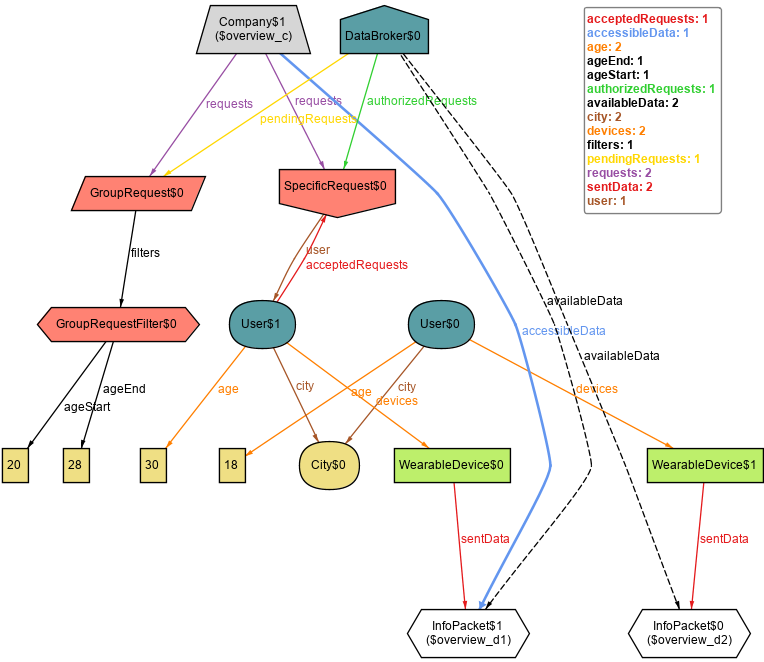
\includegraphics[width=\linewidth]{alloy_overview.png}
	\caption{Overview of the Alloy model}
	\label{fig:alloy_overview}
\end{figure}

An overview of the modeled world can be viewed in the image above. There is a company who made two requests: one GroupRequest that filters for users between 20 and 28 years old, that grants no data access since it has not been authorized by the system - here modeled by the entity DataBroker - as it is still a pendingRequest, and one SpecificRequest for User1 that the user accepted, and as such is represented in a relation of authorizedRequests with DataBroker. This means that the company has access to all the data sent by the devices of User1, represented as InfoPacket, as can be seen by the relation accessibleData between such InfoPackets and the company. The relation availableData between InfoPackets and DataBroker simply means that the system has received and stored such data and is available for companies to request or access it.
\newpage

\subsubsection{Overview with group request}

\begin{figure}[h!]
	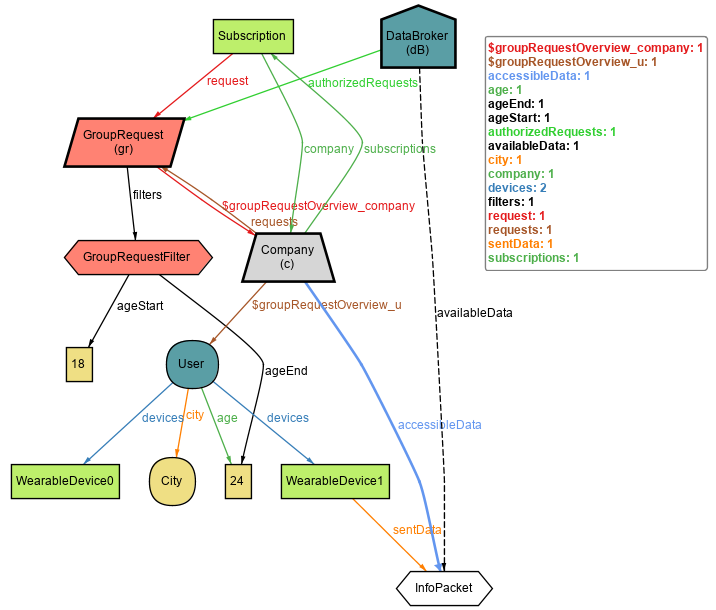
\includegraphics[width=\linewidth]{alloy_groupRequestOverview.png}
	\caption{Overview of the Alloy model with a group request for user data}
	\label{fig:alloy_groupRequestOverview}
\end{figure}

Here is represented a group request that has been authorized. This just filters for users between 18 and 24 years old and grants access to these user's data for the company. Since the only user in the model is 24 years old, all data sent from his devices is accessible. Also, as modeled, the company has subscribed to this request, so it will receive new data as soon as it is produced by the user; subscriptions can be made with SpecificRequests too.
\newpage

\subsubsection{Data request}

\begin{figure}[h!]
	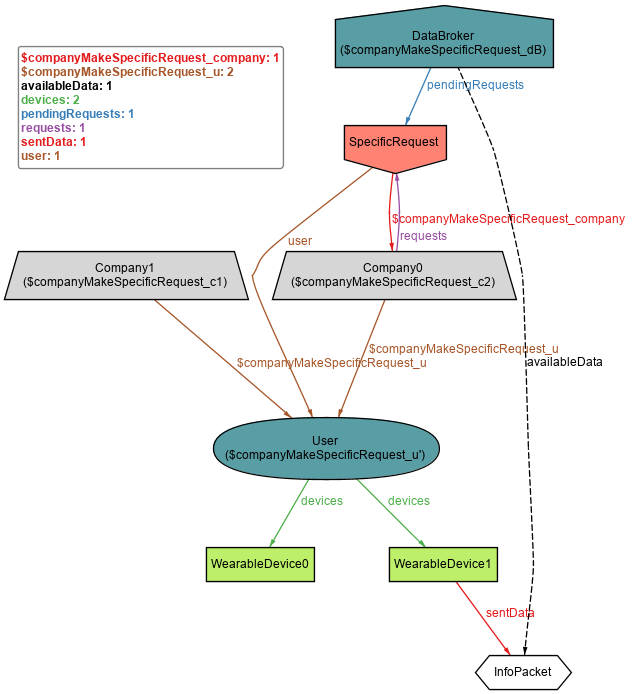
\includegraphics[width=\linewidth]{alloy_companyRequest.png}
	\caption{Overview of the Alloy model with a company forwarding a request for a user's data}
	\label{fig:alloy_companyRequest}
\end{figure}

Here is modeled the forwarding of a request for data access from a company. At the moment of the arrival of such request, Company1 is the company in the past, while Company0 is the company in the present; Company1 has no requests associated to it, while Company0 has one request for User's data, but the user hasn't accepted it yes, and as such his data is not accessible to the company.
\newpage

\subsubsection{Data request approval}

\begin{figure}[h!]
	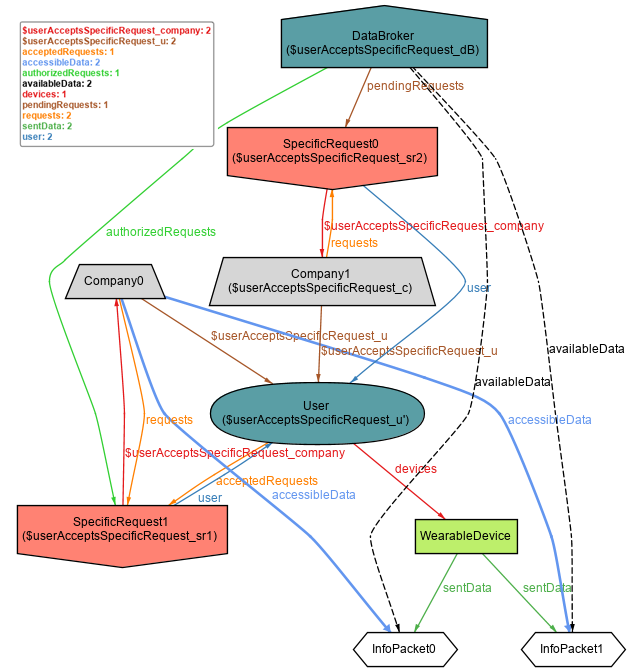
\includegraphics[width=\linewidth]{alloy_userAcceptsRequest.png}
	\caption{Overview of the Alloy model with a user accepting a request for data}
	\label{fig:alloy_userAcceptsRequest}
\end{figure}

Here is modeled one possible follow up to the situation of the previous section: now that the user has accepted to give his data to the company that made the request, his data is accessible for the company. Company1 and SpecificRequest0 are the entities of the previous section, while Company0 and SpecificRequest0 are the entities after the user's approval.
\newpage

\subsubsection{Final notes on alloy model and results}

In the previous sections of overview, some entities that were irrelevant to the analyzed situation have been hidden for clarity. The constraints on the predicates serve only to generate a meaningful and not knotty visual representation; more complex examples of the model can be generated altering these.

Following are the results the Alloy software generated.

\begin{figure}[h!]
	\centering
	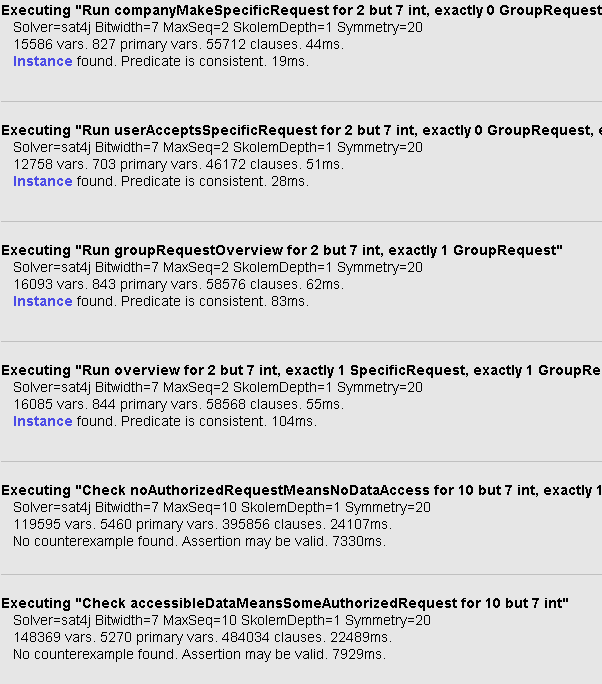
\includegraphics[scale=.5]{alloy_results.png}
	\caption{Alloy software results}
	\label{fig:alloy_results}
\end{figure}


\end{document}
